\documentclass[1p]{elsarticle_modified}
%\bibliographystyle{elsarticle-num}

%\usepackage[colorlinks]{hyperref}
%\usepackage{abbrmath_seonhwa} %\Abb, \Ascr, \Acal ,\Abf, \Afrak
\usepackage{amsfonts}
\usepackage{amssymb}
\usepackage{amsmath}
\usepackage{amsthm}
\usepackage{scalefnt}
\usepackage{amsbsy}
\usepackage{kotex}
\usepackage{caption}
\usepackage{subfig}
\usepackage{color}
\usepackage{graphicx}
\usepackage{xcolor} %% white, black, red, green, blue, cyan, magenta, yellow
\usepackage{float}
\usepackage{setspace}
\usepackage{hyperref}

\usepackage{tikz}
\usetikzlibrary{arrows}

\usepackage{multirow}
\usepackage{array} % fixed length table
\usepackage{hhline}

%%%%%%%%%%%%%%%%%%%%%
\makeatletter
\renewcommand*\env@matrix[1][\arraystretch]{%
	\edef\arraystretch{#1}%
	\hskip -\arraycolsep
	\let\@ifnextchar\new@ifnextchar
	\array{*\c@MaxMatrixCols c}}
\makeatother %https://tex.stackexchange.com/questions/14071/how-can-i-increase-the-line-spacing-in-a-matrix
%%%%%%%%%%%%%%%

\usepackage[normalem]{ulem}

\newcommand{\msout}[1]{\ifmmode\text{\sout{\ensuremath{#1}}}\else\sout{#1}\fi}
%SOURCE: \msout is \stkout macro in https://tex.stackexchange.com/questions/20609/strikeout-in-math-mode

\newcommand{\cancel}[1]{
	\ifmmode
	{\color{red}\msout{#1}}
	\else
	{\color{red}\sout{#1}}
	\fi
}

\newcommand{\add}[1]{
	{\color{blue}\uwave{#1}}
}

\newcommand{\replace}[2]{
	\ifmmode
	{\color{red}\msout{#1}}{\color{blue}\uwave{#2}}
	\else
	{\color{red}\sout{#1}}{\color{blue}\uwave{#2}}
	\fi
}

\newcommand{\Sol}{\mathcal{S}} %segment
\newcommand{\D}{D} %diagram
\newcommand{\A}{\mathcal{A}} %arc


%%%%%%%%%%%%%%%%%%%%%%%%%%%%%5 test

\def\sl{\operatorname{\textup{SL}}(2,\Cbb)}
\def\psl{\operatorname{\textup{PSL}}(2,\Cbb)}
\def\quan{\mkern 1mu \triangleright \mkern 1mu}

\theoremstyle{definition}
\newtheorem{thm}{Theorem}[section]
\newtheorem{prop}[thm]{Proposition}
\newtheorem{lem}[thm]{Lemma}
\newtheorem{ques}[thm]{Question}
\newtheorem{cor}[thm]{Corollary}
\newtheorem{defn}[thm]{Definition}
\newtheorem{exam}[thm]{Example}
\newtheorem{rmk}[thm]{Remark}
\newtheorem{alg}[thm]{Algorithm}

\newcommand{\I}{\sqrt{-1}}
\begin{document}

%\begin{frontmatter}
%
%\title{Boundary parabolic representations of knots up to 8 crossings}
%
%%% Group authors per affiliation:
%\author{Yunhi Cho} 
%\address{Department of Mathematics, University of Seoul, Seoul, Korea}
%\ead{yhcho@uos.ac.kr}
%
%
%\author{Seonhwa Kim} %\fnref{s_kim}}
%\address{Center for Geometry and Physics, Institute for Basic Science, Pohang, 37673, Korea}
%\ead{ryeona17@ibs.re.kr}
%
%\author{Hyuk Kim}
%\address{Department of Mathematical Sciences, Seoul National University, Seoul 08826, Korea}
%\ead{hyukkim@snu.ac.kr}
%
%\author{Seokbeom Yoon}
%\address{Department of Mathematical Sciences, Seoul National University, Seoul, 08826,  Korea}
%\ead{sbyoon15@snu.ac.kr}
%
%\begin{abstract}
%We find all boundary parabolic representation of knots up to 8 crossings.
%
%\end{abstract}
%\begin{keyword}
%    \MSC[2010] 57M25 
%\end{keyword}
%
%\end{frontmatter}

%\linenumbers
%\tableofcontents
%
\newcommand\colored[1]{\textcolor{white}{\rule[-0.35ex]{0.8em}{1.4ex}}\kern-0.8em\color{red} #1}%
%\newcommand\colored[1]{\textcolor{white}{ #1}\kern-2.17ex	\textcolor{white}{ #1}\kern-1.81ex	\textcolor{white}{ #1}\kern-2.15ex\color{red}#1	}

{\Large $\underline{11n_{108}~(K11n_{108})}$}

\setlength{\tabcolsep}{10pt}
\renewcommand{\arraystretch}{1.6}
\vspace{1cm}\begin{tabular}{m{100pt}>{\centering\arraybackslash}m{274pt}}
\multirow{5}{120pt}{
	\centering
	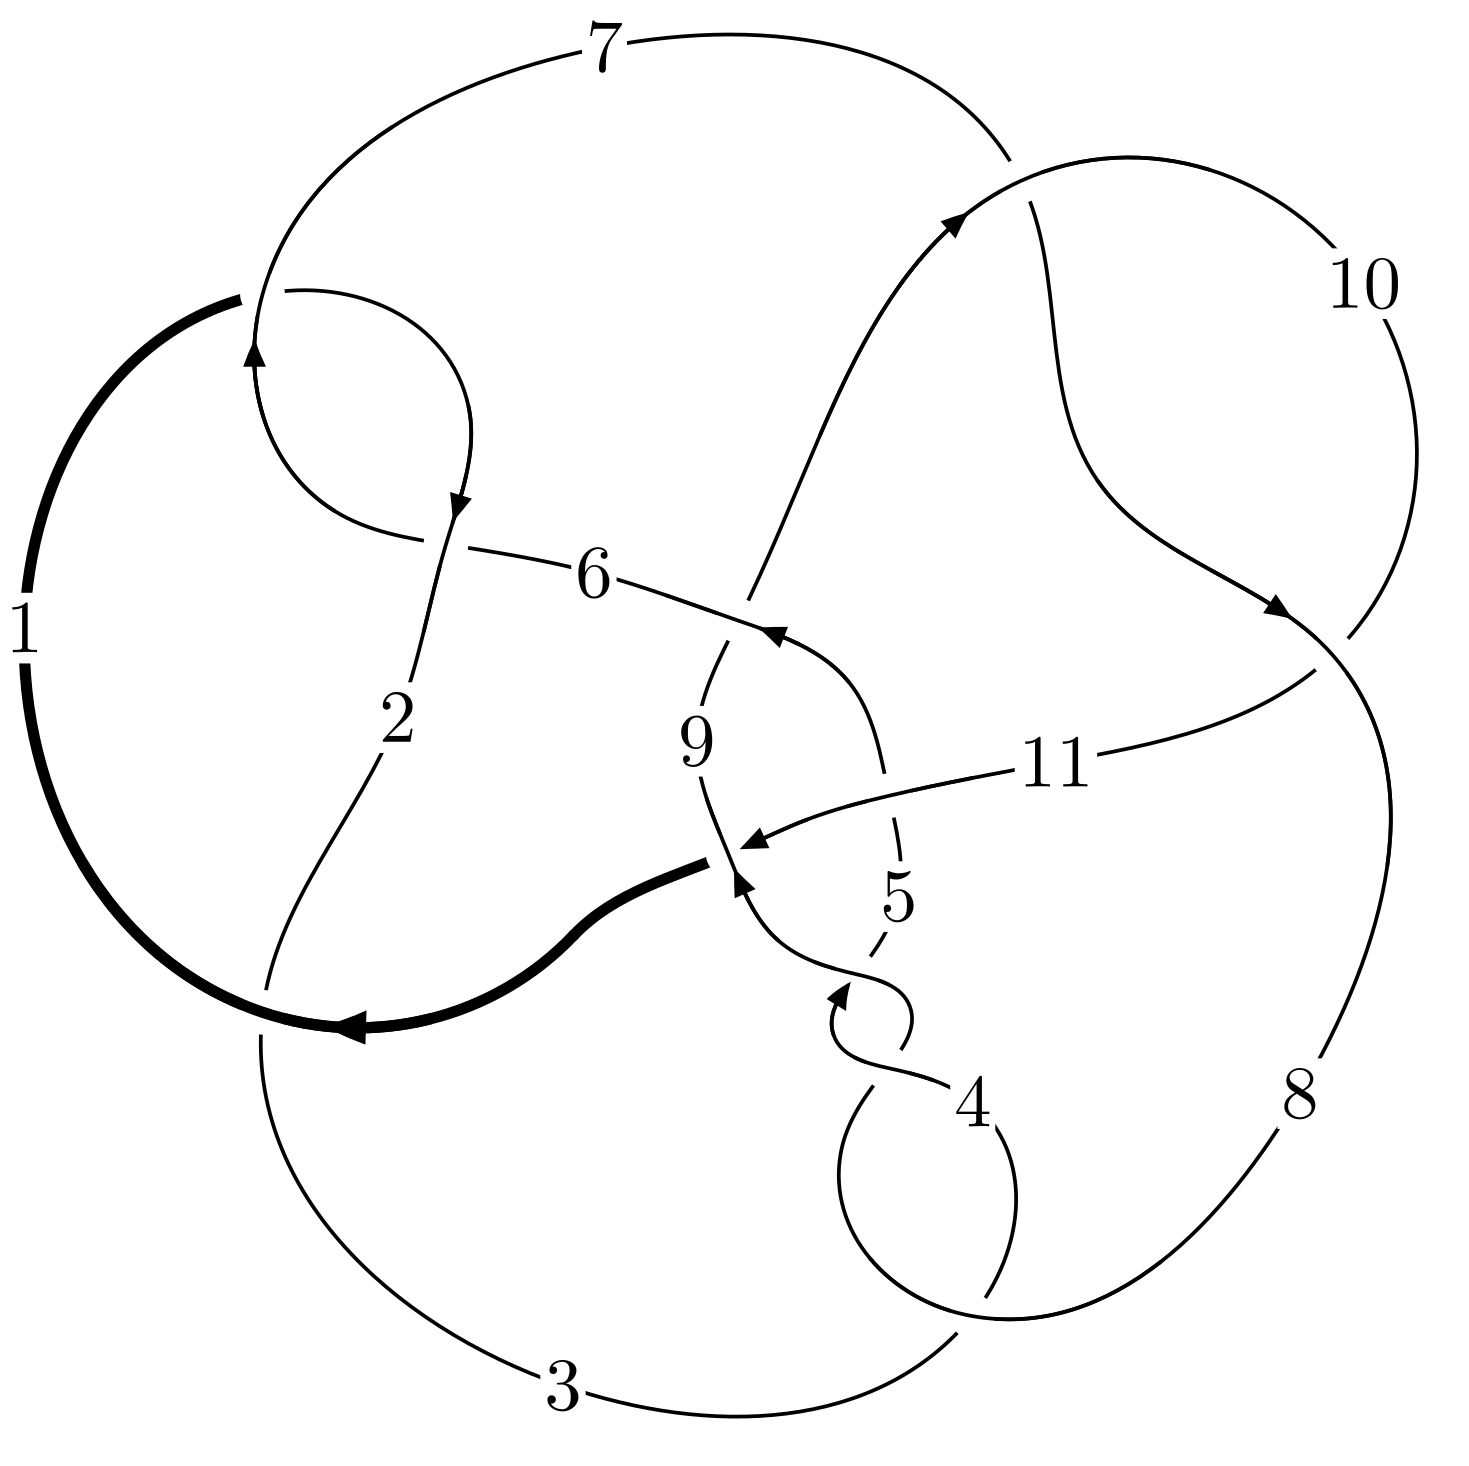
\includegraphics[width=112pt]{../../../GIT/diagram.site/Diagrams/png/724_11n_108.png}\\
\ \ \ A knot diagram\footnotemark}&
\allowdisplaybreaks
\textbf{Linearized knot diagam} \\
\cline{2-2}
 &
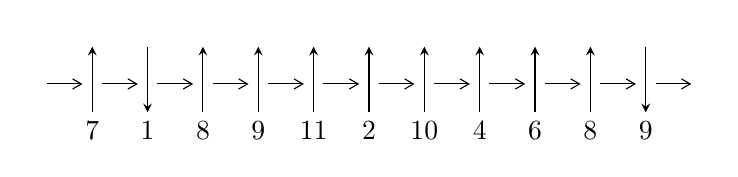
\begin{tikzpicture}[x=20pt, y=17pt]
	% nodes
	\node (C0) at (0, 0) {};
	\node (C1) at (1, 0) {};
	\node (C1U) at (1, +1) {};
	\node (C1D) at (1, -1) {7};

	\node (C2) at (2, 0) {};
	\node (C2U) at (2, +1) {};
	\node (C2D) at (2, -1) {1};

	\node (C3) at (3, 0) {};
	\node (C3U) at (3, +1) {};
	\node (C3D) at (3, -1) {8};

	\node (C4) at (4, 0) {};
	\node (C4U) at (4, +1) {};
	\node (C4D) at (4, -1) {9};

	\node (C5) at (5, 0) {};
	\node (C5U) at (5, +1) {};
	\node (C5D) at (5, -1) {11};

	\node (C6) at (6, 0) {};
	\node (C6U) at (6, +1) {};
	\node (C6D) at (6, -1) {2};

	\node (C7) at (7, 0) {};
	\node (C7U) at (7, +1) {};
	\node (C7D) at (7, -1) {10};

	\node (C8) at (8, 0) {};
	\node (C8U) at (8, +1) {};
	\node (C8D) at (8, -1) {4};

	\node (C9) at (9, 0) {};
	\node (C9U) at (9, +1) {};
	\node (C9D) at (9, -1) {6};

	\node (C10) at (10, 0) {};
	\node (C10U) at (10, +1) {};
	\node (C10D) at (10, -1) {8};

	\node (C11) at (11, 0) {};
	\node (C11U) at (11, +1) {};
	\node (C11D) at (11, -1) {9};
	\node (C12) at (12, 0) {};

	% arrows
	\draw[->,>={angle 60}]
	(C0) edge (C1) (C1) edge (C2) (C2) edge (C3) (C3) edge (C4) (C4) edge (C5) (C5) edge (C6) (C6) edge (C7) (C7) edge (C8) (C8) edge (C9) (C9) edge (C10) (C10) edge (C11) (C11) edge (C12) ;	\draw[->,>=stealth]
	(C1D) edge (C1U) (C2U) edge (C2D) (C3D) edge (C3U) (C4D) edge (C4U) (C5D) edge (C5U) (C6D) edge (C6U) (C7D) edge (C7U) (C8D) edge (C8U) (C9D) edge (C9U) (C10D) edge (C10U) (C11U) edge (C11D) ;
	\end{tikzpicture} \\
\hhline{~~} \\& 
\textbf{Solving Sequence} \\ \cline{2-2} 
 &
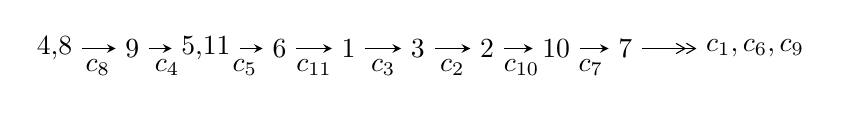
\begin{tikzpicture}[x=25pt, y=7pt]
	% node
	\node (A0) at (-1/8, 0) {4,8};
	\node (A1) at (1, 0) {9};
	\node (A2) at (33/16, 0) {5,11};
	\node (A3) at (25/8, 0) {6};
	\node (A4) at (33/8, 0) {1};
	\node (A5) at (41/8, 0) {3};
	\node (A6) at (49/8, 0) {2};
	\node (A7) at (57/8, 0) {10};
	\node (A8) at (65/8, 0) {7};
	\node (C1) at (1/2, -1) {$c_{8}$};
	\node (C2) at (3/2, -1) {$c_{4}$};
	\node (C3) at (21/8, -1) {$c_{5}$};
	\node (C4) at (29/8, -1) {$c_{11}$};
	\node (C5) at (37/8, -1) {$c_{3}$};
	\node (C6) at (45/8, -1) {$c_{2}$};
	\node (C7) at (53/8, -1) {$c_{10}$};
	\node (C8) at (61/8, -1) {$c_{7}$};
	\node (A9) at (10, 0) {$c_{1},c_{6},c_{9}$};

	% edge
	\draw[->,>=stealth]	
	(A0) edge (A1) (A1) edge (A2) (A2) edge (A3) (A3) edge (A4) (A4) edge (A5) (A5) edge (A6) (A6) edge (A7) (A7) edge (A8) ;
	\draw[->>,>={angle 60}]	
	(A8) edge (A9);
\end{tikzpicture} \\ 

\end{tabular} \\

\footnotetext{
The image of knot diagram is generated by the software ``\textbf{Draw programme}" developed by Andrew Bartholomew(\url{http://www.layer8.co.uk/maths/draw/index.htm\#Running-draw}), where we modified some parts for our purpose(\url{https://github.com/CATsTAILs/LinksPainter}).
}\phantom \\ \newline 
\centering \textbf{Ideals for irreducible components\footnotemark of $X_{\text{par}}$} 
 
\begin{align*}
I^u_{1}&=\langle 
-4.49684\times10^{62} u^{47}+2.31669\times10^{62} u^{46}+\cdots+7.77951\times10^{62} b-8.70495\times10^{63},\\
\phantom{I^u_{1}}&\phantom{= \langle  }8.71448\times10^{63} u^{47}-2.39101\times10^{63} u^{46}+\cdots+8.55746\times10^{63} a+4.29322\times10^{64},\;u^{48}- u^{47}+\cdots+16 u-11\rangle \\
I^u_{2}&=\langle 
u^{10}-4 u^8- u^7+7 u^6+3 u^5-9 u^4-2 u^3+6 u^2+b,\\
\phantom{I^u_{2}}&\phantom{= \langle  }2 u^{10}-10 u^8-2 u^7+21 u^6+8 u^5-29 u^4-9 u^3+26 u^2+a+2 u-7,\\
\phantom{I^u_{2}}&\phantom{= \langle  }u^{12}-5 u^{10}- u^9+11 u^8+4 u^7-16 u^6-5 u^5+15 u^4+2 u^3-6 u^2+1\rangle \\
\\
\end{align*}
\raggedright * 2 irreducible components of $\dim_{\mathbb{C}}=0$, with total 60 representations.\\
\footnotetext{All coefficients of polynomials are rational numbers. But the coefficients are sometimes approximated in decimal forms when there is not enough margin.}
\newpage
\renewcommand{\arraystretch}{1}
\centering \section*{I. $I^u_{1}= \langle -4.50\times10^{62} u^{47}+2.32\times10^{62} u^{46}+\cdots+7.78\times10^{62} b-8.70\times10^{63},\;8.71\times10^{63} u^{47}-2.39\times10^{63} u^{46}+\cdots+8.56\times10^{63} a+4.29\times10^{64},\;u^{48}- u^{47}+\cdots+16 u-11 \rangle$}
\flushleft \textbf{(i) Arc colorings}\\
\begin{tabular}{m{7pt} m{180pt} m{7pt} m{180pt} }
\flushright $a_{4}=$&$\begin{pmatrix}0\\u\end{pmatrix}$ \\
\flushright $a_{8}=$&$\begin{pmatrix}1\\0\end{pmatrix}$ \\
\flushright $a_{9}=$&$\begin{pmatrix}1\\- u^2\end{pmatrix}$ \\
\flushright $a_{5}=$&$\begin{pmatrix}u\\- u^3+u\end{pmatrix}$ \\
\flushright $a_{11}=$&$\begin{pmatrix}-1.01835 u^{47}+0.279406 u^{46}+\cdots+6.57363 u-5.01693\\0.578037 u^{47}-0.297794 u^{46}+\cdots+2.06984 u+11.1896\end{pmatrix}$ \\
\flushright $a_{6}=$&$\begin{pmatrix}-1.01567 u^{47}+0.683761 u^{46}+\cdots-1.11353 u-14.1587\\-0.0891298 u^{47}-0.145158 u^{46}+\cdots+6.89698 u+1.47011\end{pmatrix}$ \\
\flushright $a_{1}=$&$\begin{pmatrix}-0.866912 u^{47}+0.322213 u^{46}+\cdots+3.88254 u-8.07815\\0.221406 u^{47}-0.178838 u^{46}+\cdots+3.51193 u+9.05291\end{pmatrix}$ \\
\flushright $a_{3}=$&$\begin{pmatrix}- u\\u\end{pmatrix}$ \\
\flushright $a_{2}=$&$\begin{pmatrix}-1.06034 u^{47}+0.621352 u^{46}+\cdots+3.40978 u-11.7196\\0.128714 u^{47}-0.148448 u^{46}+\cdots-0.760314 u+0.405016\end{pmatrix}$ \\
\flushright $a_{10}=$&$\begin{pmatrix}-1.59639 u^{47}+0.577200 u^{46}+\cdots+4.50378 u-16.2065\\0.578037 u^{47}-0.297794 u^{46}+\cdots+2.06984 u+11.1896\end{pmatrix}$ \\
\flushright $a_{7}=$&$\begin{pmatrix}-0.0768387 u^{47}-0.280256 u^{46}+\cdots-3.25826 u+6.11664\\-0.0786313 u^{47}+0.170391 u^{46}+\cdots+3.31403 u-5.72912\end{pmatrix}$\\ \flushright $a_{7}=$&$\begin{pmatrix}-0.0768387 u^{47}-0.280256 u^{46}+\cdots-3.25826 u+6.11664\\-0.0786313 u^{47}+0.170391 u^{46}+\cdots+3.31403 u-5.72912\end{pmatrix}$\\&\end{tabular}
\flushleft \textbf{(ii) Obstruction class $= -1$}\\~\\
\flushleft \textbf{(iii) Cusp Shapes $= -0.320053 u^{47}-0.920029 u^{46}+\cdots+14.1517 u+26.9488$}\\~\\
\newpage\renewcommand{\arraystretch}{1}
\flushleft \textbf{(iv) u-Polynomials at the component}\newline \\
\begin{tabular}{m{50pt}|m{274pt}}
Crossings & \hspace{64pt}u-Polynomials at each crossing \\
\hline $$\begin{aligned}c_{1},c_{6}\end{aligned}$$&$\begin{aligned}
&u^{48}+12 u^{46}+\cdots- u+1
\end{aligned}$\\
\hline $$\begin{aligned}c_{2}\end{aligned}$$&$\begin{aligned}
&u^{48}+24 u^{47}+\cdots+13 u+1
\end{aligned}$\\
\hline $$\begin{aligned}c_{3},c_{4},c_{8}\end{aligned}$$&$\begin{aligned}
&u^{48}+u^{47}+\cdots-16 u-11
\end{aligned}$\\
\hline $$\begin{aligned}c_{5}\end{aligned}$$&$\begin{aligned}
&u^{48}+3 u^{47}+\cdots-14 u+1
\end{aligned}$\\
\hline $$\begin{aligned}c_{7},c_{10}\end{aligned}$$&$\begin{aligned}
&u^{48}- u^{47}+\cdots+268 u-119
\end{aligned}$\\
\hline $$\begin{aligned}c_{9}\end{aligned}$$&$\begin{aligned}
&u^{48}- u^{47}+\cdots+10 u-27
\end{aligned}$\\
\hline $$\begin{aligned}c_{11}\end{aligned}$$&$\begin{aligned}
&u^{48}-5 u^{47}+\cdots-22 u+1
\end{aligned}$\\
\hline
\end{tabular}\\~\\
\newpage\renewcommand{\arraystretch}{1}
\flushleft \textbf{(v) Riley Polynomials at the component}\newline \\
\begin{tabular}{m{50pt}|m{274pt}}
Crossings & \hspace{64pt}Riley Polynomials at each crossing \\
\hline $$\begin{aligned}c_{1},c_{6}\end{aligned}$$&$\begin{aligned}
&y^{48}+24 y^{47}+\cdots+13 y+1
\end{aligned}$\\
\hline $$\begin{aligned}c_{2}\end{aligned}$$&$\begin{aligned}
&y^{48}+8 y^{47}+\cdots-71 y+1
\end{aligned}$\\
\hline $$\begin{aligned}c_{3},c_{4},c_{8}\end{aligned}$$&$\begin{aligned}
&y^{48}-17 y^{47}+\cdots-2302 y+121
\end{aligned}$\\
\hline $$\begin{aligned}c_{5}\end{aligned}$$&$\begin{aligned}
&y^{48}+35 y^{47}+\cdots-126 y+1
\end{aligned}$\\
\hline $$\begin{aligned}c_{7},c_{10}\end{aligned}$$&$\begin{aligned}
&y^{48}-25 y^{47}+\cdots-291260 y+14161
\end{aligned}$\\
\hline $$\begin{aligned}c_{9}\end{aligned}$$&$\begin{aligned}
&y^{48}-19 y^{47}+\cdots-6904 y+729
\end{aligned}$\\
\hline $$\begin{aligned}c_{11}\end{aligned}$$&$\begin{aligned}
&y^{48}-37 y^{47}+\cdots+18 y+1
\end{aligned}$\\
\hline
\end{tabular}\\~\\
\newpage\flushleft \textbf{(vi) Complex Volumes and Cusp Shapes}
$$\begin{array}{c|c|c}  
\text{Solutions to }I^u_{1}& \I (\text{vol} + \sqrt{-1}CS) & \text{Cusp shape}\\
 \hline 
\begin{aligned}
u &= -0.541870 + 0.901222 I \\
a &= \phantom{-}0.024980 + 0.703983 I \\
b &= \phantom{-}0.816951 + 0.697564 I\end{aligned}
 & -5.53120 + 0.07674 I & \phantom{-}3.78825 - 1.36866 I \\ \hline\begin{aligned}
u &= -0.541870 - 0.901222 I \\
a &= \phantom{-}0.024980 - 0.703983 I \\
b &= \phantom{-}0.816951 - 0.697564 I\end{aligned}
 & -5.53120 - 0.07674 I & \phantom{-}3.78825 + 1.36866 I \\ \hline\begin{aligned}
u &= -0.869571 + 0.293240 I \\
a &= \phantom{-}0.127295 + 0.324289 I \\
b &= -1.41833 - 0.31833 I\end{aligned}
 & \phantom{-}3.26073 + 2.43030 I & \phantom{-}10.07781 - 2.10293 I \\ \hline\begin{aligned}
u &= -0.869571 - 0.293240 I \\
a &= \phantom{-}0.127295 - 0.324289 I \\
b &= -1.41833 + 0.31833 I\end{aligned}
 & \phantom{-}3.26073 - 2.43030 I & \phantom{-}10.07781 + 2.10293 I \\ \hline\begin{aligned}
u &= \phantom{-}0.883071 + 0.696886 I \\
a &= \phantom{-}0.586523 - 1.138810 I \\
b &= -0.304793 - 0.919600 I\end{aligned}
 & -2.06429 + 2.66223 I & \phantom{-}9.42585 - 6.21325 I \\ \hline\begin{aligned}
u &= \phantom{-}0.883071 - 0.696886 I \\
a &= \phantom{-}0.586523 + 1.138810 I \\
b &= -0.304793 + 0.919600 I\end{aligned}
 & -2.06429 - 2.66223 I & \phantom{-}9.42585 + 6.21325 I \\ \hline\begin{aligned}
u &= \phantom{-}0.843476 + 0.745354 I \\
a &= \phantom{-}0.486746 - 1.003540 I \\
b &= \phantom{-}0.111927 - 0.997408 I\end{aligned}
 & -2.19332 + 2.77840 I & \phantom{-}8.82502 - 3.26643 I \\ \hline\begin{aligned}
u &= \phantom{-}0.843476 - 0.745354 I \\
a &= \phantom{-}0.486746 + 1.003540 I \\
b &= \phantom{-}0.111927 + 0.997408 I\end{aligned}
 & -2.19332 - 2.77840 I & \phantom{-}8.82502 + 3.26643 I \\ \hline\begin{aligned}
u &= -0.702040 + 0.493195 I \\
a &= \phantom{-}0.76028 - 2.18802 I \\
b &= \phantom{-}0.951952 + 0.007910 I\end{aligned}
 & \phantom{-}3.52678 - 2.80965 I & \phantom{-}12.72101 + 4.52739 I \\ \hline\begin{aligned}
u &= -0.702040 - 0.493195 I \\
a &= \phantom{-}0.76028 + 2.18802 I \\
b &= \phantom{-}0.951952 - 0.007910 I\end{aligned}
 & \phantom{-}3.52678 + 2.80965 I & \phantom{-}12.72101 - 4.52739 I\\
 \hline 
 \end{array}$$\newpage$$\begin{array}{c|c|c}  
\text{Solutions to }I^u_{1}& \I (\text{vol} + \sqrt{-1}CS) & \text{Cusp shape}\\
 \hline 
\begin{aligned}
u &= \phantom{-}0.741649 + 0.369863 I \\
a &= -0.35152 - 1.72739 I \\
b &= -1.046450 - 0.878314 I\end{aligned}
 & \phantom{-}2.97315 + 6.07189 I & \phantom{-}11.5551 - 10.8395 I \\ \hline\begin{aligned}
u &= \phantom{-}0.741649 - 0.369863 I \\
a &= -0.35152 + 1.72739 I \\
b &= -1.046450 + 0.878314 I\end{aligned}
 & \phantom{-}2.97315 - 6.07189 I & \phantom{-}11.5551 + 10.8395 I \\ \hline\begin{aligned}
u &= -0.684846 + 0.951602 I \\
a &= -0.519439 - 0.379915 I \\
b &= -1.025990 - 0.559251 I\end{aligned}
 & -0.10143 + 2.03024 I & \phantom{-}9.27605 - 1.57972 I \\ \hline\begin{aligned}
u &= -0.684846 - 0.951602 I \\
a &= -0.519439 + 0.379915 I \\
b &= -1.025990 + 0.559251 I\end{aligned}
 & -0.10143 - 2.03024 I & \phantom{-}9.27605 + 1.57972 I \\ \hline\begin{aligned}
u &= \phantom{-}1.048110 + 0.559665 I \\
a &= \phantom{-}0.76825 - 1.24356 I \\
b &= -0.594486 - 0.287588 I\end{aligned}
 & -1.85237 + 2.17126 I & \phantom{-}11.26403 + 0. I\phantom{ +0.000000I} \\ \hline\begin{aligned}
u &= \phantom{-}1.048110 - 0.559665 I \\
a &= \phantom{-}0.76825 + 1.24356 I \\
b &= -0.594486 + 0.287588 I\end{aligned}
 & -1.85237 - 2.17126 I & \phantom{-}11.26403 + 0. I\phantom{ +0.000000I} \\ \hline\begin{aligned}
u &= -0.690139 + 0.360388 I \\
a &= -0.72752 + 1.24362 I \\
b &= -1.089830 + 0.609642 I\end{aligned}
 & \phantom{-}3.63018 - 0.51155 I & \phantom{-}11.50496 + 4.41570 I \\ \hline\begin{aligned}
u &= -0.690139 - 0.360388 I \\
a &= -0.72752 - 1.24362 I \\
b &= -1.089830 - 0.609642 I\end{aligned}
 & \phantom{-}3.63018 + 0.51155 I & \phantom{-}11.50496 - 4.41570 I \\ \hline\begin{aligned}
u &= \phantom{-}0.748525\phantom{ +0.000000I} \\
a &= -2.51365\phantom{ +0.000000I} \\
b &= \phantom{-}1.31936\phantom{ +0.000000I}\end{aligned}
 & \phantom{-}5.55263\phantom{ +0.000000I} & \phantom{-}20.1450\phantom{ +0.000000I} \\ \hline\begin{aligned}
u &= -0.587154 + 0.447682 I \\
a &= -1.33591 - 2.09829 I \\
b &= \phantom{-}1.297980 - 0.296087 I\end{aligned}
 & \phantom{-}2.15454 - 5.46033 I & \phantom{-}6.95643 + 10.69062 I\\
 \hline 
 \end{array}$$\newpage$$\begin{array}{c|c|c}  
\text{Solutions to }I^u_{1}& \I (\text{vol} + \sqrt{-1}CS) & \text{Cusp shape}\\
 \hline 
\begin{aligned}
u &= -0.587154 - 0.447682 I \\
a &= -1.33591 + 2.09829 I \\
b &= \phantom{-}1.297980 + 0.296087 I\end{aligned}
 & \phantom{-}2.15454 + 5.46033 I & \phantom{-}6.95643 - 10.69062 I \\ \hline\begin{aligned}
u &= \phantom{-}0.377726 + 0.619690 I \\
a &= \phantom{-}0.599599 - 1.043790 I \\
b &= -0.047506 - 0.807730 I\end{aligned}
 & -2.18331 + 1.63548 I & \phantom{-}3.97796 - 4.36559 I \\ \hline\begin{aligned}
u &= \phantom{-}0.377726 - 0.619690 I \\
a &= \phantom{-}0.599599 + 1.043790 I \\
b &= -0.047506 + 0.807730 I\end{aligned}
 & -2.18331 - 1.63548 I & \phantom{-}3.97796 + 4.36559 I \\ \hline\begin{aligned}
u &= -0.902068 + 0.916115 I \\
a &= \phantom{-}0.512066 + 0.717598 I \\
b &= \phantom{-}0.44776 + 1.37089 I\end{aligned}
 & -4.30258 - 7.07120 I & \phantom{-}7.00000 + 6.78102 I \\ \hline\begin{aligned}
u &= -0.902068 - 0.916115 I \\
a &= \phantom{-}0.512066 - 0.717598 I \\
b &= \phantom{-}0.44776 - 1.37089 I\end{aligned}
 & -4.30258 + 7.07120 I & \phantom{-}7.00000 - 6.78102 I \\ \hline\begin{aligned}
u &= \phantom{-}0.659900 + 0.253316 I \\
a &= \phantom{-}0.97673 + 2.73037 I \\
b &= \phantom{-}0.801186 - 0.190096 I\end{aligned}
 & \phantom{-}2.78226 - 3.51974 I & \phantom{-}11.16150 + 1.38253 I \\ \hline\begin{aligned}
u &= \phantom{-}0.659900 - 0.253316 I \\
a &= \phantom{-}0.97673 - 2.73037 I \\
b &= \phantom{-}0.801186 + 0.190096 I\end{aligned}
 & \phantom{-}2.78226 + 3.51974 I & \phantom{-}11.16150 - 1.38253 I \\ \hline\begin{aligned}
u &= \phantom{-}0.640560 + 1.139710 I \\
a &= -0.470605 + 0.463131 I \\
b &= -1.104340 + 0.854023 I\end{aligned}
 & -3.03425 - 7.47849 I & \phantom{-0.000000 } 0 \\ \hline\begin{aligned}
u &= \phantom{-}0.640560 - 1.139710 I \\
a &= -0.470605 - 0.463131 I \\
b &= -1.104340 - 0.854023 I\end{aligned}
 & -3.03425 + 7.47849 I & \phantom{-0.000000 } 0 \\ \hline\begin{aligned}
u &= \phantom{-}0.904630 + 0.964964 I \\
a &= \phantom{-}0.086405 + 1.139180 I \\
b &= \phantom{-}0.865094 + 0.549237 I\end{aligned}
 & -5.42165 + 4.76380 I & \phantom{-0.000000 } 0\\
 \hline 
 \end{array}$$\newpage$$\begin{array}{c|c|c}  
\text{Solutions to }I^u_{1}& \I (\text{vol} + \sqrt{-1}CS) & \text{Cusp shape}\\
 \hline 
\begin{aligned}
u &= \phantom{-}0.904630 - 0.964964 I \\
a &= \phantom{-}0.086405 - 1.139180 I \\
b &= \phantom{-}0.865094 - 0.549237 I\end{aligned}
 & -5.42165 - 4.76380 I & \phantom{-0.000000 } 0 \\ \hline\begin{aligned}
u &= -0.981632 + 0.915325 I \\
a &= \phantom{-}0.605329 + 1.050400 I \\
b &= -0.831231 + 1.115400 I\end{aligned}
 & -4.08127 + 0.33982 I & \phantom{-0.000000 } 0 \\ \hline\begin{aligned}
u &= -0.981632 - 0.915325 I \\
a &= \phantom{-}0.605329 - 1.050400 I \\
b &= -0.831231 - 1.115400 I\end{aligned}
 & -4.08127 - 0.33982 I & \phantom{-0.000000 } 0 \\ \hline\begin{aligned}
u &= -1.089380 + 0.813811 I \\
a &= -0.29168 - 1.41143 I \\
b &= \phantom{-}1.258230 - 0.611794 I\end{aligned}
 & \phantom{-}1.11909 - 8.52957 I & \phantom{-0.000000 } 0 \\ \hline\begin{aligned}
u &= -1.089380 - 0.813811 I \\
a &= -0.29168 + 1.41143 I \\
b &= \phantom{-}1.258230 + 0.611794 I\end{aligned}
 & \phantom{-}1.11909 + 8.52957 I & \phantom{-0.000000 } 0 \\ \hline\begin{aligned}
u &= \phantom{-}0.994777 + 0.952249 I \\
a &= -0.355078 + 0.290456 I \\
b &= -0.602542 + 0.470290 I\end{aligned}
 & -5.15741 + 2.22291 I & \phantom{-0.000000 } 0 \\ \hline\begin{aligned}
u &= \phantom{-}0.994777 - 0.952249 I \\
a &= -0.355078 - 0.290456 I \\
b &= -0.602542 - 0.470290 I\end{aligned}
 & -5.15741 - 2.22291 I & \phantom{-0.000000 } 0 \\ \hline\begin{aligned}
u &= \phantom{-}0.504319 + 0.352823 I \\
a &= \phantom{-}0.390749 - 0.726369 I \\
b &= -1.63711 + 0.11804 I\end{aligned}
 & \phantom{-}3.91125 + 1.34687 I & \phantom{-}8.42551 - 6.39280 I \\ \hline\begin{aligned}
u &= \phantom{-}0.504319 - 0.352823 I \\
a &= \phantom{-}0.390749 + 0.726369 I \\
b &= -1.63711 - 0.11804 I\end{aligned}
 & \phantom{-}3.91125 - 1.34687 I & \phantom{-}8.42551 + 6.39280 I \\ \hline\begin{aligned}
u &= -1.208410 + 0.710850 I \\
a &= \phantom{-}0.774025 + 1.048360 I \\
b &= -1.106840 + 0.481324 I\end{aligned}
 & -3.44366 - 6.15745 I & \phantom{-0.000000 } 0\\
 \hline 
 \end{array}$$\newpage$$\begin{array}{c|c|c}  
\text{Solutions to }I^u_{1}& \I (\text{vol} + \sqrt{-1}CS) & \text{Cusp shape}\\
 \hline 
\begin{aligned}
u &= -1.208410 - 0.710850 I \\
a &= \phantom{-}0.774025 - 1.048360 I \\
b &= -1.106840 - 0.481324 I\end{aligned}
 & -3.44366 + 6.15745 I & \phantom{-0.000000 } 0 \\ \hline\begin{aligned}
u &= \phantom{-}1.40818 + 0.13200 I \\
a &= -0.772395 + 0.203916 I \\
b &= \phantom{-}1.185140 - 0.228161 I\end{aligned}
 & \phantom{-}7.19540 + 0.40564 I & \phantom{-0.000000 } 0 \\ \hline\begin{aligned}
u &= \phantom{-}1.40818 - 0.13200 I \\
a &= -0.772395 - 0.203916 I \\
b &= \phantom{-}1.185140 + 0.228161 I\end{aligned}
 & \phantom{-}7.19540 - 0.40564 I & \phantom{-0.000000 } 0 \\ \hline\begin{aligned}
u &= \phantom{-}1.18080 + 0.85198 I \\
a &= -0.443194 + 1.290850 I \\
b &= \phantom{-}1.34618 + 0.78553 I\end{aligned}
 & -1.3361 + 14.6102 I & \phantom{-0.000000 } 0 \\ \hline\begin{aligned}
u &= \phantom{-}1.18080 - 0.85198 I \\
a &= -0.443194 - 1.290850 I \\
b &= \phantom{-}1.34618 - 0.78553 I\end{aligned}
 & -1.3361 - 14.6102 I & \phantom{-0.000000 } 0 \\ \hline\begin{aligned}
u &= -0.475453\phantom{ +0.000000I} \\
a &= \phantom{-}0.423852\phantom{ +0.000000I} \\
b &= -0.331940\phantom{ +0.000000I}\end{aligned}
 & \phantom{-}0.656820\phantom{ +0.000000I} & \phantom{-}15.2640\phantom{ +0.000000I} \\ \hline\begin{aligned}
u &= -1.56662 + 0.07941 I \\
a &= -0.523086 - 0.170729 I \\
b &= \phantom{-}0.733336 + 0.437414 I\end{aligned}
 & \phantom{-}5.39976 + 3.46453 I & \phantom{-0.000000 } 0 \\ \hline\begin{aligned}
u &= -1.56662 - 0.07941 I \\
a &= -0.523086 + 0.170729 I \\
b &= \phantom{-}0.733336 - 0.437414 I\end{aligned}
 & \phantom{-}5.39976 - 3.46453 I & \phantom{-0.000000 } 0\\
 \hline 
 \end{array}$$\newpage\newpage\renewcommand{\arraystretch}{1}
\centering \section*{II. $I^u_{2}= \langle u^{10}-4 u^8+\cdots+6 u^2+b,\;2 u^{10}-10 u^8+\cdots+a-7,\;u^{12}-5 u^{10}+\cdots-6 u^2+1 \rangle$}
\flushleft \textbf{(i) Arc colorings}\\
\begin{tabular}{m{7pt} m{180pt} m{7pt} m{180pt} }
\flushright $a_{4}=$&$\begin{pmatrix}0\\u\end{pmatrix}$ \\
\flushright $a_{8}=$&$\begin{pmatrix}1\\0\end{pmatrix}$ \\
\flushright $a_{9}=$&$\begin{pmatrix}1\\- u^2\end{pmatrix}$ \\
\flushright $a_{5}=$&$\begin{pmatrix}u\\- u^3+u\end{pmatrix}$ \\
\flushright $a_{11}=$&$\begin{pmatrix}-2 u^{10}+10 u^8+2 u^7-21 u^6-8 u^5+29 u^4+9 u^3-26 u^2-2 u+7\\- u^{10}+4 u^8+u^7-7 u^6-3 u^5+9 u^4+2 u^3-6 u^2\end{pmatrix}$ \\
\flushright $a_{6}=$&$\begin{pmatrix}-5 u^{11}+23 u^9+\cdots+10 u-2\\u^{11}-5 u^9- u^8+11 u^7+4 u^6-16 u^5-5 u^4+14 u^3+2 u^2-5 u\end{pmatrix}$ \\
\flushright $a_{1}=$&$\begin{pmatrix}- u^{10}+5 u^8+u^7-11 u^6-4 u^5+16 u^4+5 u^3-15 u^2-2 u+5\\- u^{10}+5 u^8+u^7-10 u^6-4 u^5+13 u^4+4 u^3-10 u^2+1\end{pmatrix}$ \\
\flushright $a_{3}=$&$\begin{pmatrix}- u\\u\end{pmatrix}$ \\
\flushright $a_{2}=$&$\begin{pmatrix}-4 u^{11}+18 u^9+\cdots+4 u-2\\3 u^{11}- u^{10}+\cdots-9 u+2\end{pmatrix}$ \\
\flushright $a_{10}=$&$\begin{pmatrix}- u^{10}+6 u^8+u^7-14 u^6-5 u^5+20 u^4+7 u^3-20 u^2-2 u+7\\- u^{10}+4 u^8+u^7-7 u^6-3 u^5+9 u^4+2 u^3-6 u^2\end{pmatrix}$ \\
\flushright $a_{7}=$&$\begin{pmatrix}- u^{11}+2 u^{10}+\cdots+3 u-8\\u^{10}-5 u^8- u^7+10 u^6+4 u^5-13 u^4-4 u^3+11 u^2-1\end{pmatrix}$\\ \flushright $a_{7}=$&$\begin{pmatrix}- u^{11}+2 u^{10}+\cdots+3 u-8\\u^{10}-5 u^8- u^7+10 u^6+4 u^5-13 u^4-4 u^3+11 u^2-1\end{pmatrix}$\\&\end{tabular}
\flushleft \textbf{(ii) Obstruction class $= 1$}\\~\\
\flushleft \textbf{(iii) Cusp Shapes $= -2 u^{10}+3 u^9+7 u^8-8 u^7-17 u^6+12 u^5+31 u^4-14 u^3-24 u^2+2 u+19$}\\~\\
\newpage\renewcommand{\arraystretch}{1}
\flushleft \textbf{(iv) u-Polynomials at the component}\newline \\
\begin{tabular}{m{50pt}|m{274pt}}
Crossings & \hspace{64pt}u-Polynomials at each crossing \\
\hline $$\begin{aligned}c_{1}\end{aligned}$$&$\begin{aligned}
&u^{12}+u^{11}+\cdots+u+1
\end{aligned}$\\
\hline $$\begin{aligned}c_{2}\end{aligned}$$&$\begin{aligned}
&u^{12}+7 u^{11}+\cdots+7 u+1
\end{aligned}$\\
\hline $$\begin{aligned}c_{3},c_{4}\end{aligned}$$&$\begin{aligned}
&u^{12}-5 u^{10}+u^9+11 u^8-4 u^7-16 u^6+5 u^5+15 u^4-2 u^3-6 u^2+1
\end{aligned}$\\
\hline $$\begin{aligned}c_{5}\end{aligned}$$&$\begin{aligned}
&u^{12}+u^{10}-3 u^9-2 u^7+4 u^6- u^5+3 u^4+u^3-4 u^2+1
\end{aligned}$\\
\hline $$\begin{aligned}c_{6}\end{aligned}$$&$\begin{aligned}
&u^{12}- u^{11}+\cdots- u+1
\end{aligned}$\\
\hline $$\begin{aligned}c_{7}\end{aligned}$$&$\begin{aligned}
&u^{12}+2 u^{11}+\cdots+2 u+1
\end{aligned}$\\
\hline $$\begin{aligned}c_{8}\end{aligned}$$&$\begin{aligned}
&u^{12}-5 u^{10}- u^9+11 u^8+4 u^7-16 u^6-5 u^5+15 u^4+2 u^3-6 u^2+1
\end{aligned}$\\
\hline $$\begin{aligned}c_{9}\end{aligned}$$&$\begin{aligned}
&u^{12}-4 u^{10}+u^9+3 u^8- u^7+4 u^6-2 u^5-3 u^3+u^2+1
\end{aligned}$\\
\hline $$\begin{aligned}c_{10}\end{aligned}$$&$\begin{aligned}
&u^{12}-2 u^{11}+\cdots-2 u+1
\end{aligned}$\\
\hline $$\begin{aligned}c_{11}\end{aligned}$$&$\begin{aligned}
&u^{12}+2 u^{11}- u^{10}-2 u^9+3 u^8+u^7+u^6+7 u^5+2 u^4+2 u^2+1
\end{aligned}$\\
\hline
\end{tabular}\\~\\
\newpage\renewcommand{\arraystretch}{1}
\flushleft \textbf{(v) Riley Polynomials at the component}\newline \\
\begin{tabular}{m{50pt}|m{274pt}}
Crossings & \hspace{64pt}Riley Polynomials at each crossing \\
\hline $$\begin{aligned}c_{1},c_{6}\end{aligned}$$&$\begin{aligned}
&y^{12}+7 y^{11}+\cdots+7 y+1
\end{aligned}$\\
\hline $$\begin{aligned}c_{2}\end{aligned}$$&$\begin{aligned}
&y^{12}+3 y^{11}+\cdots- y+1
\end{aligned}$\\
\hline $$\begin{aligned}c_{3},c_{4},c_{8}\end{aligned}$$&$\begin{aligned}
&y^{12}-10 y^{11}+\cdots-12 y+1
\end{aligned}$\\
\hline $$\begin{aligned}c_{5}\end{aligned}$$&$\begin{aligned}
&y^{12}+2 y^{11}+\cdots-8 y+1
\end{aligned}$\\
\hline $$\begin{aligned}c_{7},c_{10}\end{aligned}$$&$\begin{aligned}
&y^{12}-10 y^{11}+\cdots+2 y+1
\end{aligned}$\\
\hline $$\begin{aligned}c_{9}\end{aligned}$$&$\begin{aligned}
&y^{12}-8 y^{11}+\cdots+2 y+1
\end{aligned}$\\
\hline $$\begin{aligned}c_{11}\end{aligned}$$&$\begin{aligned}
&y^{12}-6 y^{11}+\cdots+4 y+1
\end{aligned}$\\
\hline
\end{tabular}\\~\\
\newpage\flushleft \textbf{(vi) Complex Volumes and Cusp Shapes}
$$\begin{array}{c|c|c}  
\text{Solutions to }I^u_{2}& \I (\text{vol} + \sqrt{-1}CS) & \text{Cusp shape}\\
 \hline 
\begin{aligned}
u &= \phantom{-}0.944121 + 0.586418 I \\
a &= \phantom{-}0.85764 - 1.21516 I \\
b &= -0.316252 - 0.773855 I\end{aligned}
 & -2.69108 + 2.27732 I & -0.79309 - 1.51304 I \\ \hline\begin{aligned}
u &= \phantom{-}0.944121 - 0.586418 I \\
a &= \phantom{-}0.85764 + 1.21516 I \\
b &= -0.316252 + 0.773855 I\end{aligned}
 & -2.69108 - 2.27732 I & -0.79309 + 1.51304 I \\ \hline\begin{aligned}
u &= -0.971824 + 0.903078 I \\
a &= \phantom{-}0.199108 + 0.774068 I \\
b &= -0.226863 + 0.457126 I\end{aligned}
 & -5.04286 - 3.33069 I & \phantom{-}6.48064 + 3.71539 I \\ \hline\begin{aligned}
u &= -0.971824 - 0.903078 I \\
a &= \phantom{-}0.199108 - 0.774068 I \\
b &= -0.226863 - 0.457126 I\end{aligned}
 & -5.04286 + 3.33069 I & \phantom{-}6.48064 - 3.71539 I \\ \hline\begin{aligned}
u &= -1.339700 + 0.047045 I \\
a &= -0.920911 - 0.442643 I \\
b &= \phantom{-}1.230580 + 0.195712 I\end{aligned}
 & \phantom{-}7.43656 - 1.12784 I & \phantom{-}13.7843 + 5.8074 I \\ \hline\begin{aligned}
u &= -1.339700 - 0.047045 I \\
a &= -0.920911 + 0.442643 I \\
b &= \phantom{-}1.230580 - 0.195712 I\end{aligned}
 & \phantom{-}7.43656 + 1.12784 I & \phantom{-}13.7843 - 5.8074 I \\ \hline\begin{aligned}
u &= \phantom{-}0.555310 + 0.250101 I \\
a &= \phantom{-}0.60842 - 3.02308 I \\
b &= -1.167560 - 0.430017 I\end{aligned}
 & \phantom{-}2.81163 + 4.85898 I & \phantom{-}13.04273 - 4.67018 I \\ \hline\begin{aligned}
u &= \phantom{-}0.555310 - 0.250101 I \\
a &= \phantom{-}0.60842 + 3.02308 I \\
b &= -1.167560 + 0.430017 I\end{aligned}
 & \phantom{-}2.81163 - 4.85898 I & \phantom{-}13.04273 + 4.67018 I \\ \hline\begin{aligned}
u &= \phantom{-}1.399120 + 0.104604 I \\
a &= -0.338465 + 0.499440 I \\
b &= \phantom{-}0.964221 - 0.298157 I\end{aligned}
 & \phantom{-}6.28022 - 3.33267 I & \phantom{-}14.8487 + 3.1328 I \\ \hline\begin{aligned}
u &= \phantom{-}1.399120 - 0.104604 I \\
a &= -0.338465 - 0.499440 I \\
b &= \phantom{-}0.964221 + 0.298157 I\end{aligned}
 & \phantom{-}6.28022 + 3.33267 I & \phantom{-}14.8487 - 3.1328 I\\
 \hline 
 \end{array}$$\newpage$$\begin{array}{c|c|c}  
\text{Solutions to }I^u_{2}& \I (\text{vol} + \sqrt{-1}CS) & \text{Cusp shape}\\
 \hline 
\begin{aligned}
u &= -0.587029 + 0.077244 I \\
a &= \phantom{-}0.59421 + 1.34198 I \\
b &= -1.48412 + 0.20351 I\end{aligned}
 & \phantom{-}4.36500 + 0.58143 I & \phantom{-}14.6367 + 0.1461 I \\ \hline\begin{aligned}
u &= -0.587029 - 0.077244 I \\
a &= \phantom{-}0.59421 - 1.34198 I \\
b &= -1.48412 - 0.20351 I\end{aligned}
 & \phantom{-}4.36500 - 0.58143 I & \phantom{-}14.6367 - 0.1461 I\\
 \hline 
 \end{array}$$\newpage
\newpage\renewcommand{\arraystretch}{1}
\centering \section*{ III. u-Polynomials}
\begin{tabular}{m{50pt}|m{274pt}}
Crossings & \hspace{64pt}u-Polynomials at each crossing \\
\hline $$\begin{aligned}c_{1}\end{aligned}$$&$\begin{aligned}
&(u^{12}+u^{11}+\cdots+u+1)(u^{48}+12 u^{46}+\cdots- u+1)
\end{aligned}$\\
\hline $$\begin{aligned}c_{2}\end{aligned}$$&$\begin{aligned}
&(u^{12}+7 u^{11}+\cdots+7 u+1)(u^{48}+24 u^{47}+\cdots+13 u+1)
\end{aligned}$\\
\hline $$\begin{aligned}c_{3},c_{4}\end{aligned}$$&$\begin{aligned}
&(u^{12}-5 u^{10}+u^9+11 u^8-4 u^7-16 u^6+5 u^5+15 u^4-2 u^3-6 u^2+1)\\
&\cdot(u^{48}+u^{47}+\cdots-16 u-11)
\end{aligned}$\\
\hline $$\begin{aligned}c_{5}\end{aligned}$$&$\begin{aligned}
&(u^{12}+u^{10}-3 u^9-2 u^7+4 u^6- u^5+3 u^4+u^3-4 u^2+1)\\
&\cdot(u^{48}+3 u^{47}+\cdots-14 u+1)
\end{aligned}$\\
\hline $$\begin{aligned}c_{6}\end{aligned}$$&$\begin{aligned}
&(u^{12}- u^{11}+\cdots- u+1)(u^{48}+12 u^{46}+\cdots- u+1)
\end{aligned}$\\
\hline $$\begin{aligned}c_{7}\end{aligned}$$&$\begin{aligned}
&(u^{12}+2 u^{11}+\cdots+2 u+1)(u^{48}- u^{47}+\cdots+268 u-119)
\end{aligned}$\\
\hline $$\begin{aligned}c_{8}\end{aligned}$$&$\begin{aligned}
&(u^{12}-5 u^{10}- u^9+11 u^8+4 u^7-16 u^6-5 u^5+15 u^4+2 u^3-6 u^2+1)\\
&\cdot(u^{48}+u^{47}+\cdots-16 u-11)
\end{aligned}$\\
\hline $$\begin{aligned}c_{9}\end{aligned}$$&$\begin{aligned}
&(u^{12}-4 u^{10}+u^9+3 u^8- u^7+4 u^6-2 u^5-3 u^3+u^2+1)\\
&\cdot(u^{48}- u^{47}+\cdots+10 u-27)
\end{aligned}$\\
\hline $$\begin{aligned}c_{10}\end{aligned}$$&$\begin{aligned}
&(u^{12}-2 u^{11}+\cdots-2 u+1)(u^{48}- u^{47}+\cdots+268 u-119)
\end{aligned}$\\
\hline $$\begin{aligned}c_{11}\end{aligned}$$&$\begin{aligned}
&(u^{12}+2 u^{11}- u^{10}-2 u^9+3 u^8+u^7+u^6+7 u^5+2 u^4+2 u^2+1)\\
&\cdot(u^{48}-5 u^{47}+\cdots-22 u+1)
\end{aligned}$\\
\hline
\end{tabular}\newpage\renewcommand{\arraystretch}{1}
\centering \section*{ IV. Riley Polynomials}
\begin{tabular}{m{50pt}|m{274pt}}
Crossings & \hspace{64pt}Riley Polynomials at each crossing \\
\hline $$\begin{aligned}c_{1},c_{6}\end{aligned}$$&$\begin{aligned}
&(y^{12}+7 y^{11}+\cdots+7 y+1)(y^{48}+24 y^{47}+\cdots+13 y+1)
\end{aligned}$\\
\hline $$\begin{aligned}c_{2}\end{aligned}$$&$\begin{aligned}
&(y^{12}+3 y^{11}+\cdots- y+1)(y^{48}+8 y^{47}+\cdots-71 y+1)
\end{aligned}$\\
\hline $$\begin{aligned}c_{3},c_{4},c_{8}\end{aligned}$$&$\begin{aligned}
&(y^{12}-10 y^{11}+\cdots-12 y+1)(y^{48}-17 y^{47}+\cdots-2302 y+121)
\end{aligned}$\\
\hline $$\begin{aligned}c_{5}\end{aligned}$$&$\begin{aligned}
&(y^{12}+2 y^{11}+\cdots-8 y+1)(y^{48}+35 y^{47}+\cdots-126 y+1)
\end{aligned}$\\
\hline $$\begin{aligned}c_{7},c_{10}\end{aligned}$$&$\begin{aligned}
&(y^{12}-10 y^{11}+\cdots+2 y+1)(y^{48}-25 y^{47}+\cdots-291260 y+14161)
\end{aligned}$\\
\hline $$\begin{aligned}c_{9}\end{aligned}$$&$\begin{aligned}
&(y^{12}-8 y^{11}+\cdots+2 y+1)(y^{48}-19 y^{47}+\cdots-6904 y+729)
\end{aligned}$\\
\hline $$\begin{aligned}c_{11}\end{aligned}$$&$\begin{aligned}
&(y^{12}-6 y^{11}+\cdots+4 y+1)(y^{48}-37 y^{47}+\cdots+18 y+1)
\end{aligned}$\\
\hline
\end{tabular}
\vskip 2pc
\end{document}